\documentclass[11pt]{article}
    
\usepackage{amsmath}
\usepackage{amsfonts}
\usepackage{cite}
\usepackage[letterpaper, total={6.5in, 9in}]{geometry}
\usepackage{mathpazo}
\usepackage{sourcecodepro}
\usepackage{graphicx}

\usepackage{hyperref}

\newcommand{\setcomp}[2]{\left\{ #1 \ \Big|\ #2 \right\}}
\newcommand{\rngto}[1]{1{:}#1}
\newcommand{\abs}[1]{\left| #1 \right|}
\newcommand{\absdet}[1]{\abs{#1}}
\newcommand{\dv}[1]{\mathrm{d}{#1}}
\newcommand{\Exp}{\mathrm{Exp}}
\newcommand{\vect}{\mathrm{vec}}
\newcommand{\vectu}{\mathrm{vecu}}

\begin{document}


\title{Efficient Unconstraining
  Parameter Transforms for Hamiltonian Monte Carlo}
\author{Meenal Jhajaria \\ \small Flatiron Institute 
\and Seth Axen \\ \small University of T\"ubingen 
\and Adam Haber \\ \small Weizmann Institute 
\and Sean Pinkney \\ \small Omnicom Media Group
\and Bob Carpenter \\ \small Flatiron Institute}
\date{DRAFT: \today}
\maketitle


\begin{abstract}
  \noindent
  This paper evaluates the statistical and computational
  efficiency of unconstraining parameter transforms for Hamiltonian
  Monte Carlo sampling.
\end{abstract}

\section{Introduction}

In statistical computing, we often need to compute high-dimensional
integrals over densities $\pi(x)$ (e.g., Bayesian estimation or
prediction, $p$-value calculations, etc.).  The only black-box
techniques that work for general high-dimensional integrals are
Markov chain Monte Carlo (MCMC) methods.  The most effective MCMC
method in high dimensions is Hamiltonian Monte Carlo (HMC).  HMC works
by simulating the Hamiltonian dynamics of a fictitious particle
representing the value being sampled coupled with a momentum term.

Although it's possible to write HMC samplers that work for simply
constrained values such as upper- and/or lower-bounds
\cite{neal2011mcmc} or unit vectors \cite{byrne2013geodesic}, it is
much more challenging to do the same for complex constraints such as
simplexes or positive definite matrices or for densities involving
multiple constrained values.  Instead, it is far more common to map
the constrained values to unconstrained values before sampling
\cite{}.  This presents the issue of selecting which transform to use
among an infinite set of options, which is the topic of this paper.

%Sampling algorithms play an important role in Statistics, in this case
%we refer to drawing samples from a probability density or distribution
%(not survey sampling). Monte Carlo Markov chain methods are commonly
%used for high dimensional sampling. In this paper, we look at
%Hamiltonian Monte Carlo, which uses hamiltonian dynamics to propose
%samples for the Metropolis algorithm. Bayesian Inference often uses
%parameters with constraints, but HMC optimizes on the unconstrained
%space. It is difficult to use Monte Carlo estimation on a constrained
%domain ~\cite{neal2008optimal}



\section{Transforms}

To draw samples from a distribution $p_X(x)$, defined on a constrained space $\mathcal{X}$ that can be uniquely parameterized by $n$ real degrees of freedom, we instead perform sampling in an unconstrained space $\mathcal{Y}=\mathbb{R}^m$ for $m \ge n$.

Let $f\colon \mathcal{Y} \to \mathcal{X}$ be a smooth and continuous map.
Only when $m = n$ can $f$ be bijective.
When $m > n$, multiple values of $y \in \mathcal{Y}$ may map to a given value of $x = f(y)$.
In this case, to make the function bijective, we consider an additional smooth and continuous map $g\colon \mathcal{Y} \to \mathcal{Z}$, where $\mathcal{Z}$ can be uniquely parameterized by $m - n$ real degrees of freedom.
We then define $h\colon \mathcal{Y} \to \mathcal{X} \times \mathcal{Z}: y \mapsto (f(y), g(y)) = (x, z)$.
$f$ and $g$ must be chosen so that $h$ is bijective almost-everywhere;
that is, the values of $y$ for which $h$ is non-bijective must have no probability mass.
When $h$ is non-bijective at single points, we call these singularities.
While singularities themselves are in general not a problem for sampling with MCMC, the region of a target density near the singularity tends to have high curvature.

Given a proper joint distribution with a smooth and continuous density $p_{X,Y}(x, y | \theta)$ for some parameters $\theta$, we can use the usual change of variables formula to write

\[
  p_Y(y | \theta) = p_{X,Z}(f(y), g(y) | \theta) |J_h(y)|.
\]

To sample from a target density $p_X(x | \theta)$, let $p_{X,Z}(x, z | \theta) = p_X(x | \theta) p_Z(z | x, \theta)$.
Then we must choose some proper distribution $p_Z$ that is smooth and continuous.
Given that choice, we find that
\[
  p_Y(y | \theta) = p_X(f(y) | \theta) p_Z(g(y) | f(y), \theta) |J_h(y)|.
\]

Note that when $m > n$, it is insufficient to specify a transform $h$.
One must also select a prior $p_Z$, and it is desirable to establish some general properties that a given pair $h$ and $p_Z$ should have.
In addition to the above properties, the optimal pair would
1. discard as few degrees of freedom $|m - n|$ as possible.
2. produce a $p_Z$ and $|J_y|$ and their gradients that are efficient to compute.
3. produce a $p_Y$ that is easy to sample from.

We can expand a bit on the latter point.
As a general rule, the more normal $p_Y$ is, the easier it is to sample from (REF?).
Additionally, near singularities, small perturbations to $y$ tend to result in larger changes to $h(y)$ than far from the singularity.
This warps the volume around the singularity, which causes $|J_y(y)|$ to smoothly approach infinity near the singularity.
If $m$ is large, this is generally not a problem, as the "curse of dimensionality" works in our favor, and there is exponentially more volume away from the singularity than near the singularity.
However, for low $m$, it is necessary that $p_{X,Z}$ goes to 0 near the singularity faster than $|J_y(y)|$ goes to infinity.
While $p_X$ is generally fixed by the user-specified model and may not have this necessary property, the user may then choose a $p_Z$ that has this property.

\subsection{Changes of Variables}

If $X$ is a random variable with density $p_X$ and $Y = f(X)$ for a
smooth, monotonic, bijection $f$, then
\[
  p_Y(y) = p_X(f^{-1}(y)) \absdet{J_{f^{-1}}(y)},
\]
where the Jacobian of the inverse transform is defined by
\[
  J_{f^{-1}}(y) = \frac{\partial}{\partial y} \, f^{-1}(y)
\]
and
\[
  \absdet{J_{f^{-1}}(y)}
  = \abs{\det J_{f^{-1}}(y)}.
\]

\subsection{Computing Jacobian}


To compute Jacobians of functions with matrix-valued inputs or outputs, we need to implicitly or explicitly choose for the inputs and outputs a set of coordinates with dimension equal to the number of degrees of freedom of the matrix
Unless otherwise specified, we choose the coordinates to be the vectorization of the matrix.

We define the (bijective) vectorization of a matrix $X \in \mathbb{R}^{N \times K}$ with columns $x_k$ for $k \in \{1, ..., K\}$ as the vector
\[\vect(X) = \begin{bmatrix}x_1 \\ x_2 \\ \vdots \\ x_M\end{bmatrix}\]
formed by stacking the columns of $X$.

For $X \in \mathbb{R}^{N \times K}$, let $\vectu(X)$ be the map that stacks only the parts of the columns of $X$ above and including the diagonal.
This map is sometimes called the half-vectorization and is bijective for upper-triangular or symmetric $X$.

Similarly, $\vectu_-(X)$ extracts the same elements except the diagonal.
When $X$ is strictly upper-triangular or skew-symmetric (i.e. $X = -X^\top$), then this map is bijective.

Here we introduce several strategies for computing Jacobian determinants.

The vectorization has the useful property that for all matrices $A$, $X$, and $B$, $\vect(AYB) = (B^\top \otimes A) \vect(Y)$, where $\otimes$ is the Kronecker product.
This allows us to convert expressions of matrices to expressions of vectors, from which the Jacobian can be read off.
For example, let $X = AYB$. Then $\dv{X} = A \dv{Y} B$, and $\vect(\dv{X}) = (B^\top \otimes A) \vect(\dv{Y})$, and the Jacobian is $J = B^\top \otimes A$.

\section{Unit simplex}

A unit $N$-simplex is an $N + 1$-dimensional vector of non-negative
values that sums to one.  As such, there are only $N$ degrees of
freedom, because if $x$ is an $N$-simplex, then
\[
  x_N = -(x_1 + x_2 + \cdots + x_{N-1}).
\]
Simplexes are useful for representations of multinomial probabilities
(e.g., probabilities of categories in a classification problem).

The set of unit $N$-simplexes is conventionally denoted
\[
  \Delta^N = \setcomp{x \in \mathbb{R}^{N + 1}}{\textrm{sum}(x) = 1
    \textrm{ and }
    x_n \geq 0 \textrm{ for } n \in \rngto{N}}
\]
Geometrically, an $N$-simplex is the convex closure of $N+1$ points
that are 1 in one coordinate and 0 elsewhere.  For example, the
3-simplex is the complex closure of
$\begin{bmatrix}1 & 0 & 0 \end{bmatrix},
\begin{bmatrix} 0 & 1 & 0 \end{bmatrix}$,
and $\begin{bmatrix} 0 & 0 & 1 \end{bmatrix}$.

\subsection{StickBreaking Transform}

The StickBreaking transform ican be be understood from the stick-breaking construction for Dirichlet \cite{sethurman}. Intuitively, this comprises of recursively breaking a piece $x_i$ from a stick of unit length, where the leftover stick in the $i^{th}$ iteration is $ 1 - \sum_{1}^{i}x$. Let $y = f(x)$, then we define the stick-breaking mapping $ f \colon \Delta^{N-1} \xrightarrow{\makebox[0.4cm]{$\sim$}}  R^{N-1}$, for $1 \leq i \leq N$ as:	
\[
y_i
= \mathrm{logit}(z_i) - \mbox{log}\left(\frac{1}{N-i}
   \right) \text{for break proportion} \, 
   z_i = \frac{x_i}{1 - \sum_{i' = 1}^{i-1} x_{i'}}.
\]

The inverse transform $ f^{-1} \colon R^{N-1} \xrightarrow{\makebox[0.4cm]{$\sim$}}  \Delta^{N-1}$ is defined as:
\[
x_i =
\left( 1 - \sum_{i'=1}^{i-1} x_{i'} \right) \text{for break proportion} \, z_i = \mathrm{logit}^{-1} \left( y_i
                             + \log \left( \frac{1}{N - i}
                                            \right)\right).
                                            \]
                            
An $N$ dimensional unit simplex $\Delta^{N-1}$ has $N-1$ degrees of freedom (Notice that this inverse transform only maps the first $N-1$ elements, the last element of the simplex $x_{N} = 1 - \sum_1^{N-1}{x_i}$). The Jacobian matrix for $f^{-1}$ is a lower-triangular diagonal matrix. Much like the alr transform, for the change of variables we evaluate $\mathbf{J}_{i, i}$ where $i \in 1:N-1$.
\begin{align*}
\mathbf{J}_{i, i} &= \frac{\partial x_i}{\partial y_i}
=
\frac{\partial x_i}{\partial z_i} \,
\frac{\partial z_i}{\partial y_i}\\
\mathbf{J}_{i, i} &= \left(
  1 - \sum_{k' = 1}^{k-1} x_{k'}
   \right) z_k (1 - z_k),
\end{align*}

Absolute determinant of the diagonal matrix $\mathbf{J}$ is the product of its diagonal entries:
\begin{align*}
	\abs{\, det \, \textbf{J} \,} = \prod_{i=1}^{N-1} \textbf{J}_{i,i}
\end{align*}

The correction term $p_Y(y) = p_X(f^{-1}(y))\,
\prod_{i=1}^{N-1}z_i\,(1 - z_i)\left(1 - \sum_{i'=1}^{i-1} x_{i'}\right).$
\subsection{Additive log ratio transform}

The unconstraining transform for the identified softmax is known as
the additive log ratio (ALR) transform
\cite{aitchison1982statistical}, which is a bijection
$\textrm{alr}:\Delta^{N-1} \rightarrow \mathbb{R}^{N-1}$ defined for
$x \in \Delta^{N-1}$ by
\[
  \textrm{alr}(x)
  = \begin{bmatrix}\displaystyle
    \log \frac{x_1}{x_N} \cdots \log \frac{x_{N-1}}{x_N}
  \end{bmatrix}.
\]

The inverse additive log ratio transform maps values in
$\mathbb{R}^{N-1}$ to $\Delta^{N-1}$ defined for $y \in
\mathbb{R}^{N-1}$ by
\[
  \textrm{alr}^{-1}(y)
  = \textrm{softmax}(\begin{bmatrix} y &  0 \end{bmatrix}),
\]
where for $u \in \mathbb{R}^N$,
\[
  \textrm{softmax}(u) = \frac{\exp(u)}{\textrm{sum}(\exp(u))}.
\]

To calculate the change of variables adjustment, we consider only the
first $N-1$ coordinates of the result, because the last is defined in
terms of the first $N-1$.  For convenience, we define a function 
$s:\mathbb{R}^{N-1} \rightarrow \mathbb{R}^{N-1}$ that operates on
$N-1$ unconstrained variables and returns the first $N-1$ components
of the $\textrm{alr}^{-1}(y)$, which is
defined for $y \in \mathbb{R}^{N-1}$ by
\[
  s(y) = \frac{\exp(y)}{\textrm{sum}(\exp(y)) + 1}
  = \begin{bmatrix}
    \textrm{alr}^{-1}(y)_1
    & \cdots &
    \textrm{alr}^{-1}(y)_{N-1}
    \end{bmatrix}.
\]
Given a density $p_X(x)$ defined over simplices $x \in \Delta^{N-1}$,
we can transform to a density over unconstrained parameters $y \in
\mathbb{R}^{N-1}$ by applying the inverse ALR transform and adjusting
for the change of variables, which yields
\[
  p_Y(y) = p_X(\textrm{alr}^{-1}(y)) \absdet{J_{s}(y)},
\]
where $J_{s}(y)$ is the Jacobian of the function $s$ evaluated at $y$
and $\absdet{J_s(y)}$ is the absolute value of its determinant.


\subsubsection{Softmax Transform}

To calculate the determinant of the Jacobian of the inverse transform,
we start by noting that $s = \textrm{exp} \circ \textrm{norm}$, where
$\textrm{exp}$ is the elementwise exponential function and
\textrm{norm} is defined by
\[
  \textrm{norm}(z) = \frac{z}{\textrm{sum}(z) + 1}.
\]
As such, the resulting Jacobian determinant is the product of the
Jacobian determinants of the component functions,
\[
  \absdet{J_s(y)}
  = \absdet{J_{\textrm{exp}}(y)} \absdet{J_{\textrm{norm}}(z)},
\]
where $z = \textrm{exp}(y)$.  The Jacobian for the exponential
function is diagonal, so the determinant is the product of the
diagonal of the Jacobian, which for $y \in \mathbb{R}^{N-1}$ is
\[
  \absdet{J_{\textrm{exp}}(y)} = \textrm{prod}(\exp(y)).
\]
As above, let $z = \exp(y) \in (0, \inf)^{N-1}$.  We can differentiate
$\textrm{norm}$ to derive the Jacobian,
\[
  J_{\textrm{norm}}
  = \frac{1}{1 + \textrm{sum}(z)} \mathbb{I}_{N-1}
  - \left(\frac{1}{(1 + \textrm{sum}(z))^2} \beta \right)
  \textrm{vector}_{N-1}(1)^{\top},
\]
where $\mathbb{I}_{N-1}$ is the $(N - 1) \times (N - 1)$ unit matrix and
$\textrm{vector}_{N-1}(1)$ is the $N - 1$-vector with values 1.  Using
the matrix determinant lemma,\footnote{The matrix determinant lemma
  is \[\textrm{det}(A + u v^{\top}) = (1 + v^{\top} A^{-1} u)
    \textrm{det}(A).\]}
we have
\begin{eqnarray*}
  \textrm{absdet}(J_{\textrm{norm}}(z))
  & = &
  \left(
    1
    + \textrm{vector}_{N-1}(1)^{\top}
    \left(\frac{1}{1 + \textrm{sum}(z)} \mathbb{I} \right)^{-1}
    \frac{-z}{(1 + \textrm{sum}(z))^2}
    \right)
    \ \textrm{det}\left(\frac{1}{1 + \textrm{sum}(z)} \mathbb{I}
        \right)
  \\[6pt]
  & = &
  \left(
    1 
    + \textrm{sum}\left( \frac{-(1 + \textrm{sum}(z)) z}{(1 +
        \textrm{sum}(z))^2} \right)
  \right)
        \ \left( \frac{1}{1 + \textrm{sum}(z)} \right)^{N-1}
  \\[6pt]
  & = &
        \left(1 + \textrm{sum}\left(\frac{-z}{1 + \textrm{sum}(z)} \right)\right)        
        \ \left( \frac{1}{1 + \textrm{sum}(z)} \right)^{N-1}
  \\[6pt]
  & = & \left( 1 - \textrm{sum}(\textrm{norm}(z)) \right) 
        \ \left( \frac{1}{1 + \textrm{sum}(z)} \right)^{N-1}
  \\[6pt]
  & = & \left( \frac{1}{1 + \textrm{sum}(z)} \right)^N.
\end{eqnarray*}
Thus the entire absolute determinant of the Jacobian is defined by the
product, 
\[
  \absdet{J_s(y)}
  \ = \
  \textrm{prod}(\exp(y))
  \, \left( \frac{1}{1 + \textrm{sum}(\exp(y))} \right)^N.
\]
and our final expression for densities for unconstrained $y \in
\mathbb{R}^{N-1}$ is
\[
  p_Y(y)
  = p_X(\textrm{alr}^{-1}(y))
  \, \textrm{prod}(\exp(y))
  \left( \frac{1}{1 + \textrm{sum}(\exp(y))} \right)^N
\]  

%\subsection{Softmax Transform}
%
%The softmax function can be understood from Multinomial Logistic
%Regression employed for predicting probabilities of a Categorically
%distributed variable. Geometrically it maps $R^K$ to the boundary of a
%unit K-simplex(it is simply the convex hull of $k+1$ affinely
%independent points in $R^K$. Essentially it transforms a vector of
%size K to another vector of size K where the outputs sum to 1. It is
%worth noting that the mapping is actually from $R^K$ to $R^{K-1}$, so
%when a vector of size $K$ is transformed the $K_th$ vector is simply
%$1$- sumof k-1 vectors


\subsection{Simplex softmax parameterization}

Let $\Delta^n$ indicate the unit $n$-simplex with $n$ positive
elements that sum to 1 and $\Delta^n_-$ indicate the first $n-1$
elements, from which the final element can be uniquely determined.

We define the transformation
$\phi: \mathbb{R}^{n-1} \to \Delta^n_-: y \mapsto x_-$, where
$x=\begin{pmatrix}x_- \\ \frac{1}{r}\end{pmatrix} \in \Delta^n$,
$x_i = \frac{1}{r} e^{y_i}$ for $1 \le i \le n-1$, and
$r = 1 + \sum_{i=1}^{n-1} e^{y_i}$.

First we compute the scalar derivatives:
\[
\begin{aligned}
  \frac{\mathrm{d} r}{\mathrm{d} y_j}
  &= e^{y_j} = r x_j\\
  \frac{\mathrm{d} x_i}{\mathrm{d} y_j}
  &= \delta_{ij} \frac{1}{r} e^{y_i} - \frac{1}{r^2} e^{y_i}
  \frac{\mathrm{d} r}{\mathrm{d} y_j}
  = \delta_{ij} x_i - x_i x_j, \quad 1 \le i \le n-1
\end{aligned}
\]
where
$\delta_{ij} = \begin{cases} 1 &\text{if } i = j \\ 0
  &\text{otherwise}\end{cases}$ is the Kronecker delta.

If $\mathrm{diag}(x)$ is the diagonal matrix whose diagonal are the
elements of $x$, then the Jacobian is
\[
  J = (I_{n-1} - x_- \boldsymbol{1}_{n-1}^\top) \operatorname{diag}(x_-),
\]
where $\boldsymbol{1}_n$ is the $n$-vector of ones.

Using Sylvester's determinant theorem,
$|I_{n-1} - x_- \boldsymbol{1}_{n-1}^\top| = 1 -
\boldsymbol{1}_{n-1}^\top x_- = 1 - \sum_{i=1}^{n-1} x_i = x_n$, so
$$\mathrm{correction} = |J| = x_n \prod_{i=1}^{n-1} x_i = \prod_{i=1}^{n} x_i = \exp\left(\sum_{i=1}^{n-1} y_i\right) \left(1 + \sum_{i=1}^{n-1} e^{y_i}\right)^{-n}$$


\subsection{Simplex softmax parameterization through parameter expansion}

We define the transformation
$\phi: \mathbb{R}^n \to \Delta^{n-1} \times \mathbb{R}_{>0}: y \mapsto
(x_-, r)$, where $r = \sum_{i=1}^n e^{y_i}$ and
$x_i = \frac{1}{r} e^{y_i}$ for $1 \le i \le n-1$..

First we compute the scalar derivatives:
\[
\begin{aligned}
  \frac{\mathrm{d} r}{\mathrm{d} y_j}
  &= e^{y_j} = r x_j
  \\
  \frac{\mathrm{d} x_i}{\mathrm{d} y_j}
  &= \delta_{ij} \frac{1}{r} e^{y_i} - \frac{1}{r^2} e^{y_i} \frac{\mathrm{d} r}{\mathrm{d} y_j} = \delta_{ij} x_i - x_i x_j,
\end{aligned}
\]
which corresponds to the Jacobian
\[
  J = \begin{pmatrix}I_{n-1} - x_- \boldsymbol{1}_{n-1}^\top & -x_- \\
    r \boldsymbol{1}_{n-1}^\top & r \end{pmatrix} \mathrm{diag}(x).
\]

For invertible $A$, the determinant of the block matrix
$\begin{pmatrix}A & B \\ C & D\end{pmatrix}$ is $|A| |D-CA^{-1}B|$.  A
square matrix is invertible iff its determinant is non-yero.  From the
previous section,
\[
  |I_{n-1} - x_- \boldsymbol{1}_{n-1}^\top| = x_n > 0,
\]
so the determinant of the Jacobian is
\[
  |J| = x_n \left|r + r \boldsymbol{1}_{n-1}^\top (I_{n-1} - x_-
    \boldsymbol{1}_{n-1}^\top)^{-1} x_-\right|
  \prod_{i=1}^n x_i.
\]

Let $w = (I_{n-1} - x_- \boldsymbol{1}_{n-1}^\top)^{-1} x_-$. Then,
\[
\begin{aligned}
    w - x_- \sum_{i=1}^{n-1} w_i &= x_-\\
    w &= x_- \left(1 - \sum_{i=1}^{n-1} w_i\right)\\
    \sum_{i=1}^{n-1} w_i &= \sum_{i=1}^{n-1} \left( x_- (1 - \sum_{i=1}^{n-1} w_i) \right) = \left(\sum_{i=1}^{n-1} x_i \right) \left(1 - \sum_{i=1}^{n-1} w_i\right) = (1 - x_n)  \left(1 - \sum_{i=1}^{n-1} w_i\right)\\
    \sum_{i=1}^{n-1} w_i &= \frac{1 - x_n}{x_n} = \frac{1}{x_n} - 1\\
    w &= x_- \left(1 - \left(\frac{1}{x_n} - 1\right)\right) = \frac{1}{x_n} x_-
  \end{aligned}
\]

Then
\[
  |J| = x_n r \left|1 + \frac{1}{x_n}\sum_{i=1}^{n-1} x_i\right|
  \prod_{i=1}^n x_i = r \prod_{i=1}^n x_i
\]

To keep the target distribution proper, we must select a prior
distribution $\pi(r)$ for $r$.  If we choose $r \sim \chi_n$, then the
product of the correction and the density of the prior for $r$ is
proportional to

\[
  \mathrm{correction}
  = \pi(r) |J| = r^n e^{-r^2/2} \prod_{i=1}^n x_i
  = \exp\left(\sum_{i=1}^n y_i - \frac{1}{2}\left(\sum_{i=1}^n
      e^{y_i}\right)^2\right).
\]

Alternatively, if we choose $r \sim \mathrm{Gamma}(n, 1)$, then
\[
  \mathrm{correction} = \pi(r) |J| = r^n e^{-r} \prod_{i=1}^n x_i =
  \exp\left(\sum_{i=1}^n y_i - \sum_{i=1}^n e^{y_i}\right).
\]
This latter correction is equivalent to the sampling procedure from
the Dirichlet distribution with $\alpha_i=1$, where
$z_i \sim \mathrm{Exponential}(1)$ and
$y = \frac{z}{\sum_{i=1}^n z_i}$.

Both of these corrections can be captured with the generalization
\[
  \mathrm{correction}
  = \pi(r) |J|
  = r^n e^{-r^p/p} \prod_{i=1}^n x_i
  = \exp\left(\sum_{i=1}^n y_i - \frac{1}{p} \left(\sum_{i=1}^n e^{y_i}\right)^p\right),
\]
for $p > 0$, which corresponds to $r \sim \text{Generalized-Gamma}(1, n, p)$.

\section{Results}

\begin{figure}
    \centering
    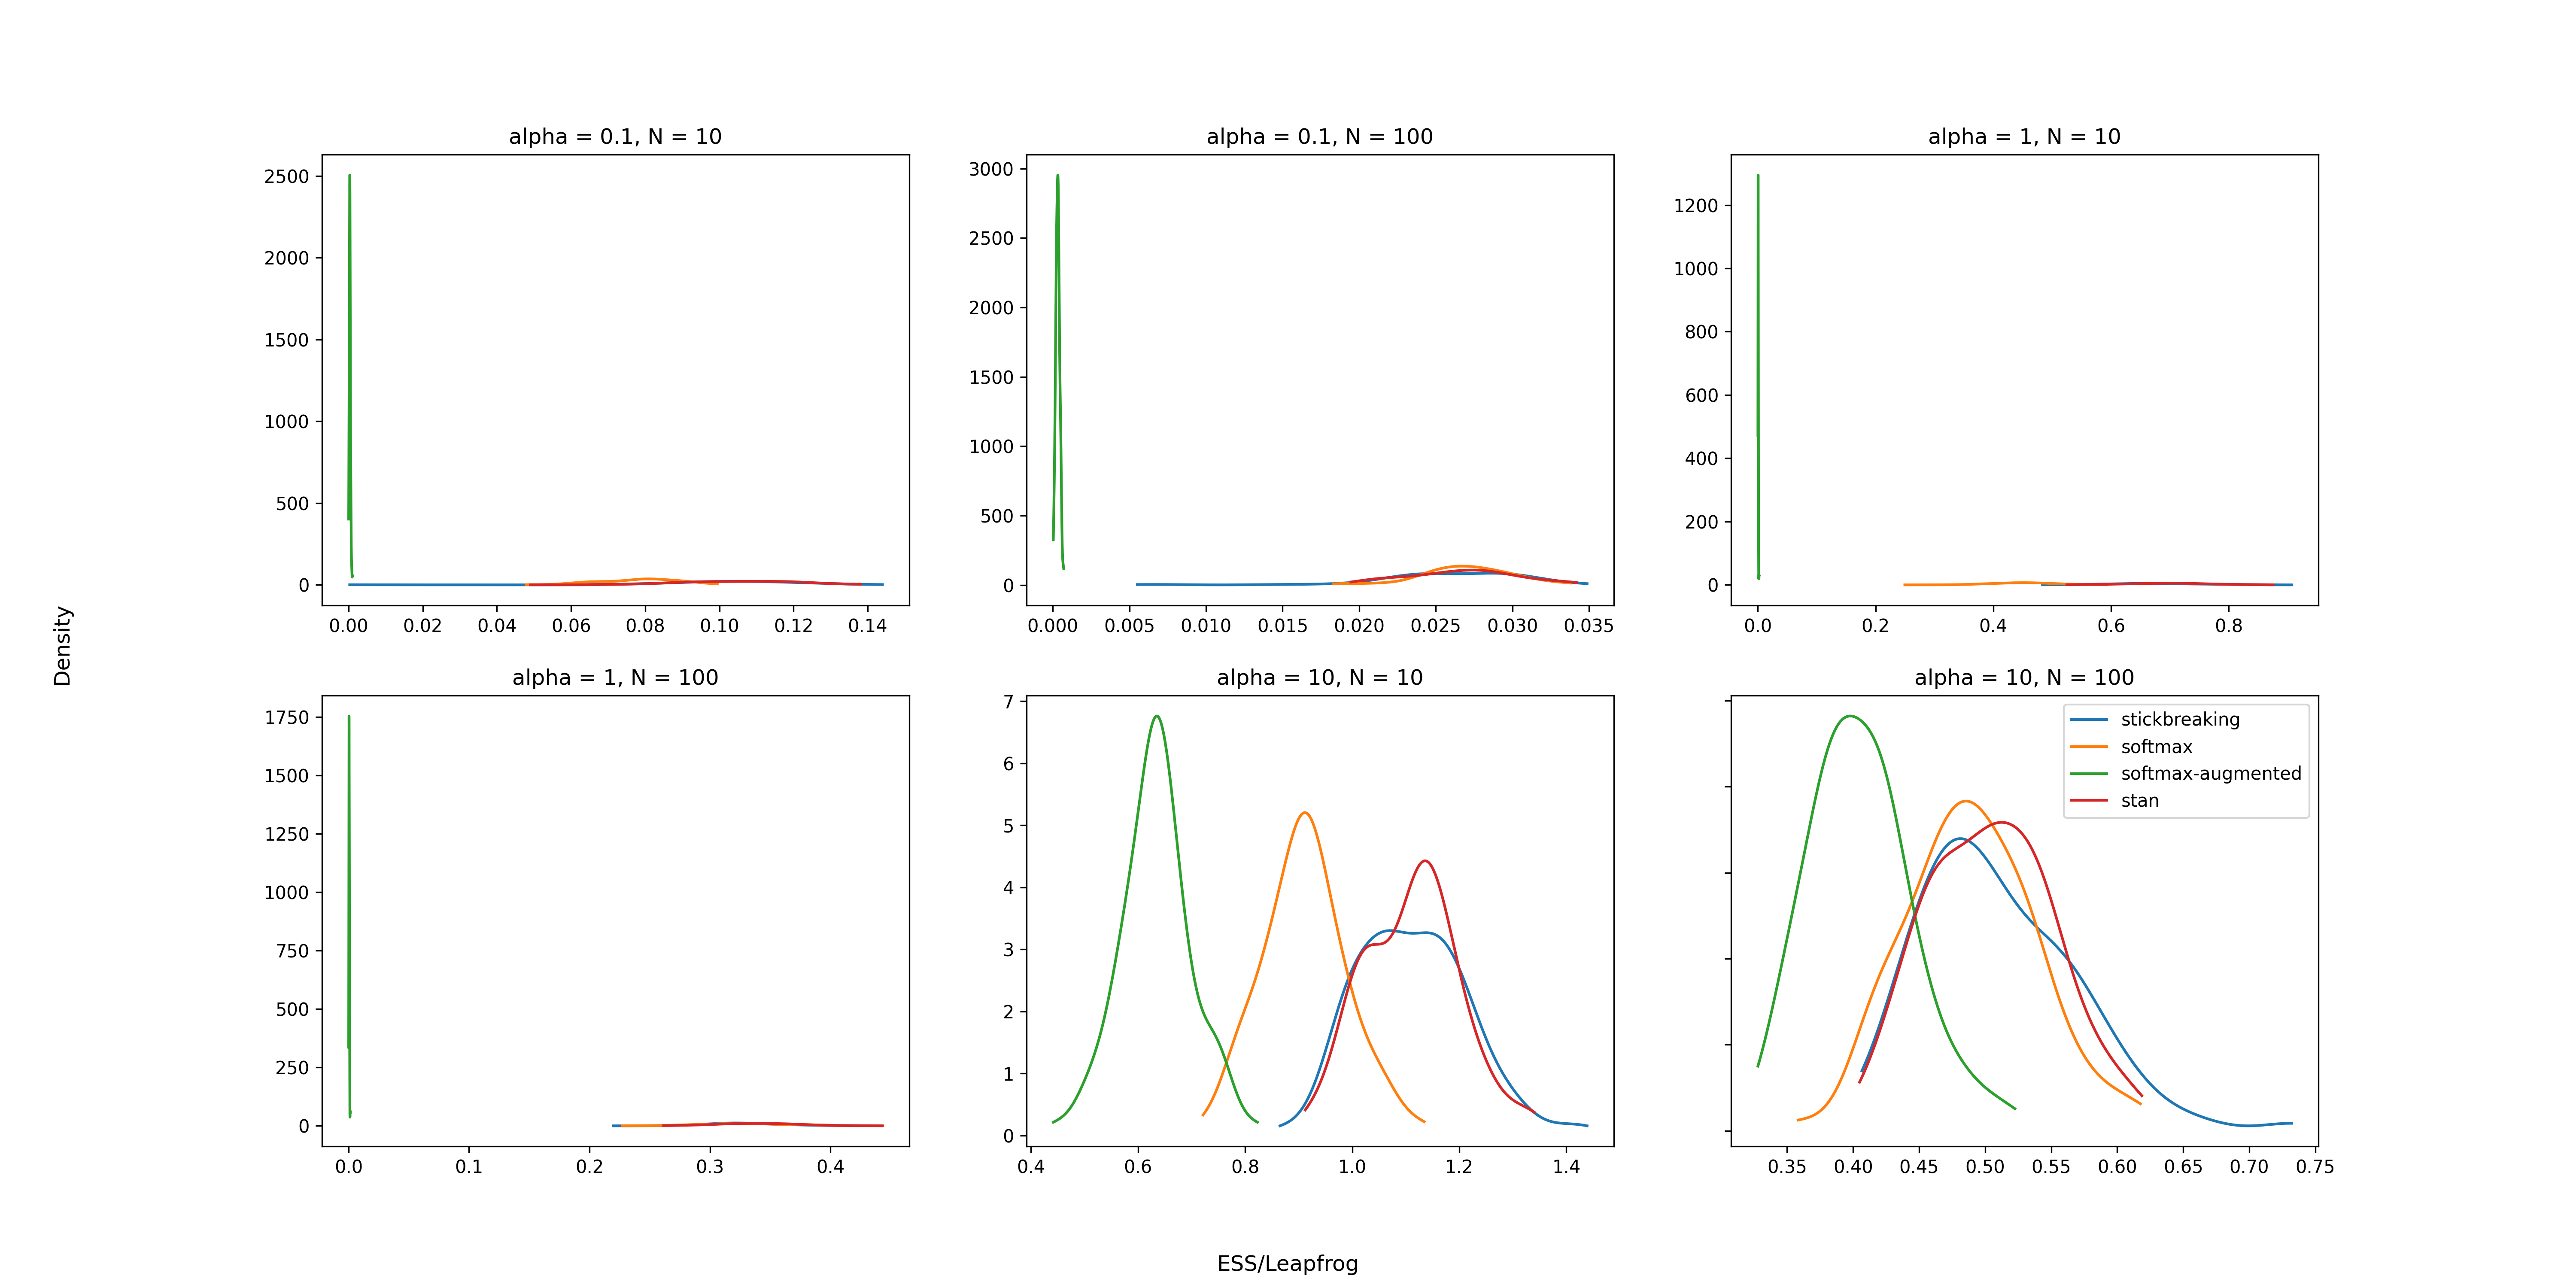
\includegraphics[width=1.2\textwidth]{figures/ess.png}
    \caption{Effective Sample Size vs Total LeapFrog Steps}
    \label{fig:hyg}
\end{figure}

\begin{figure}
    \centering
    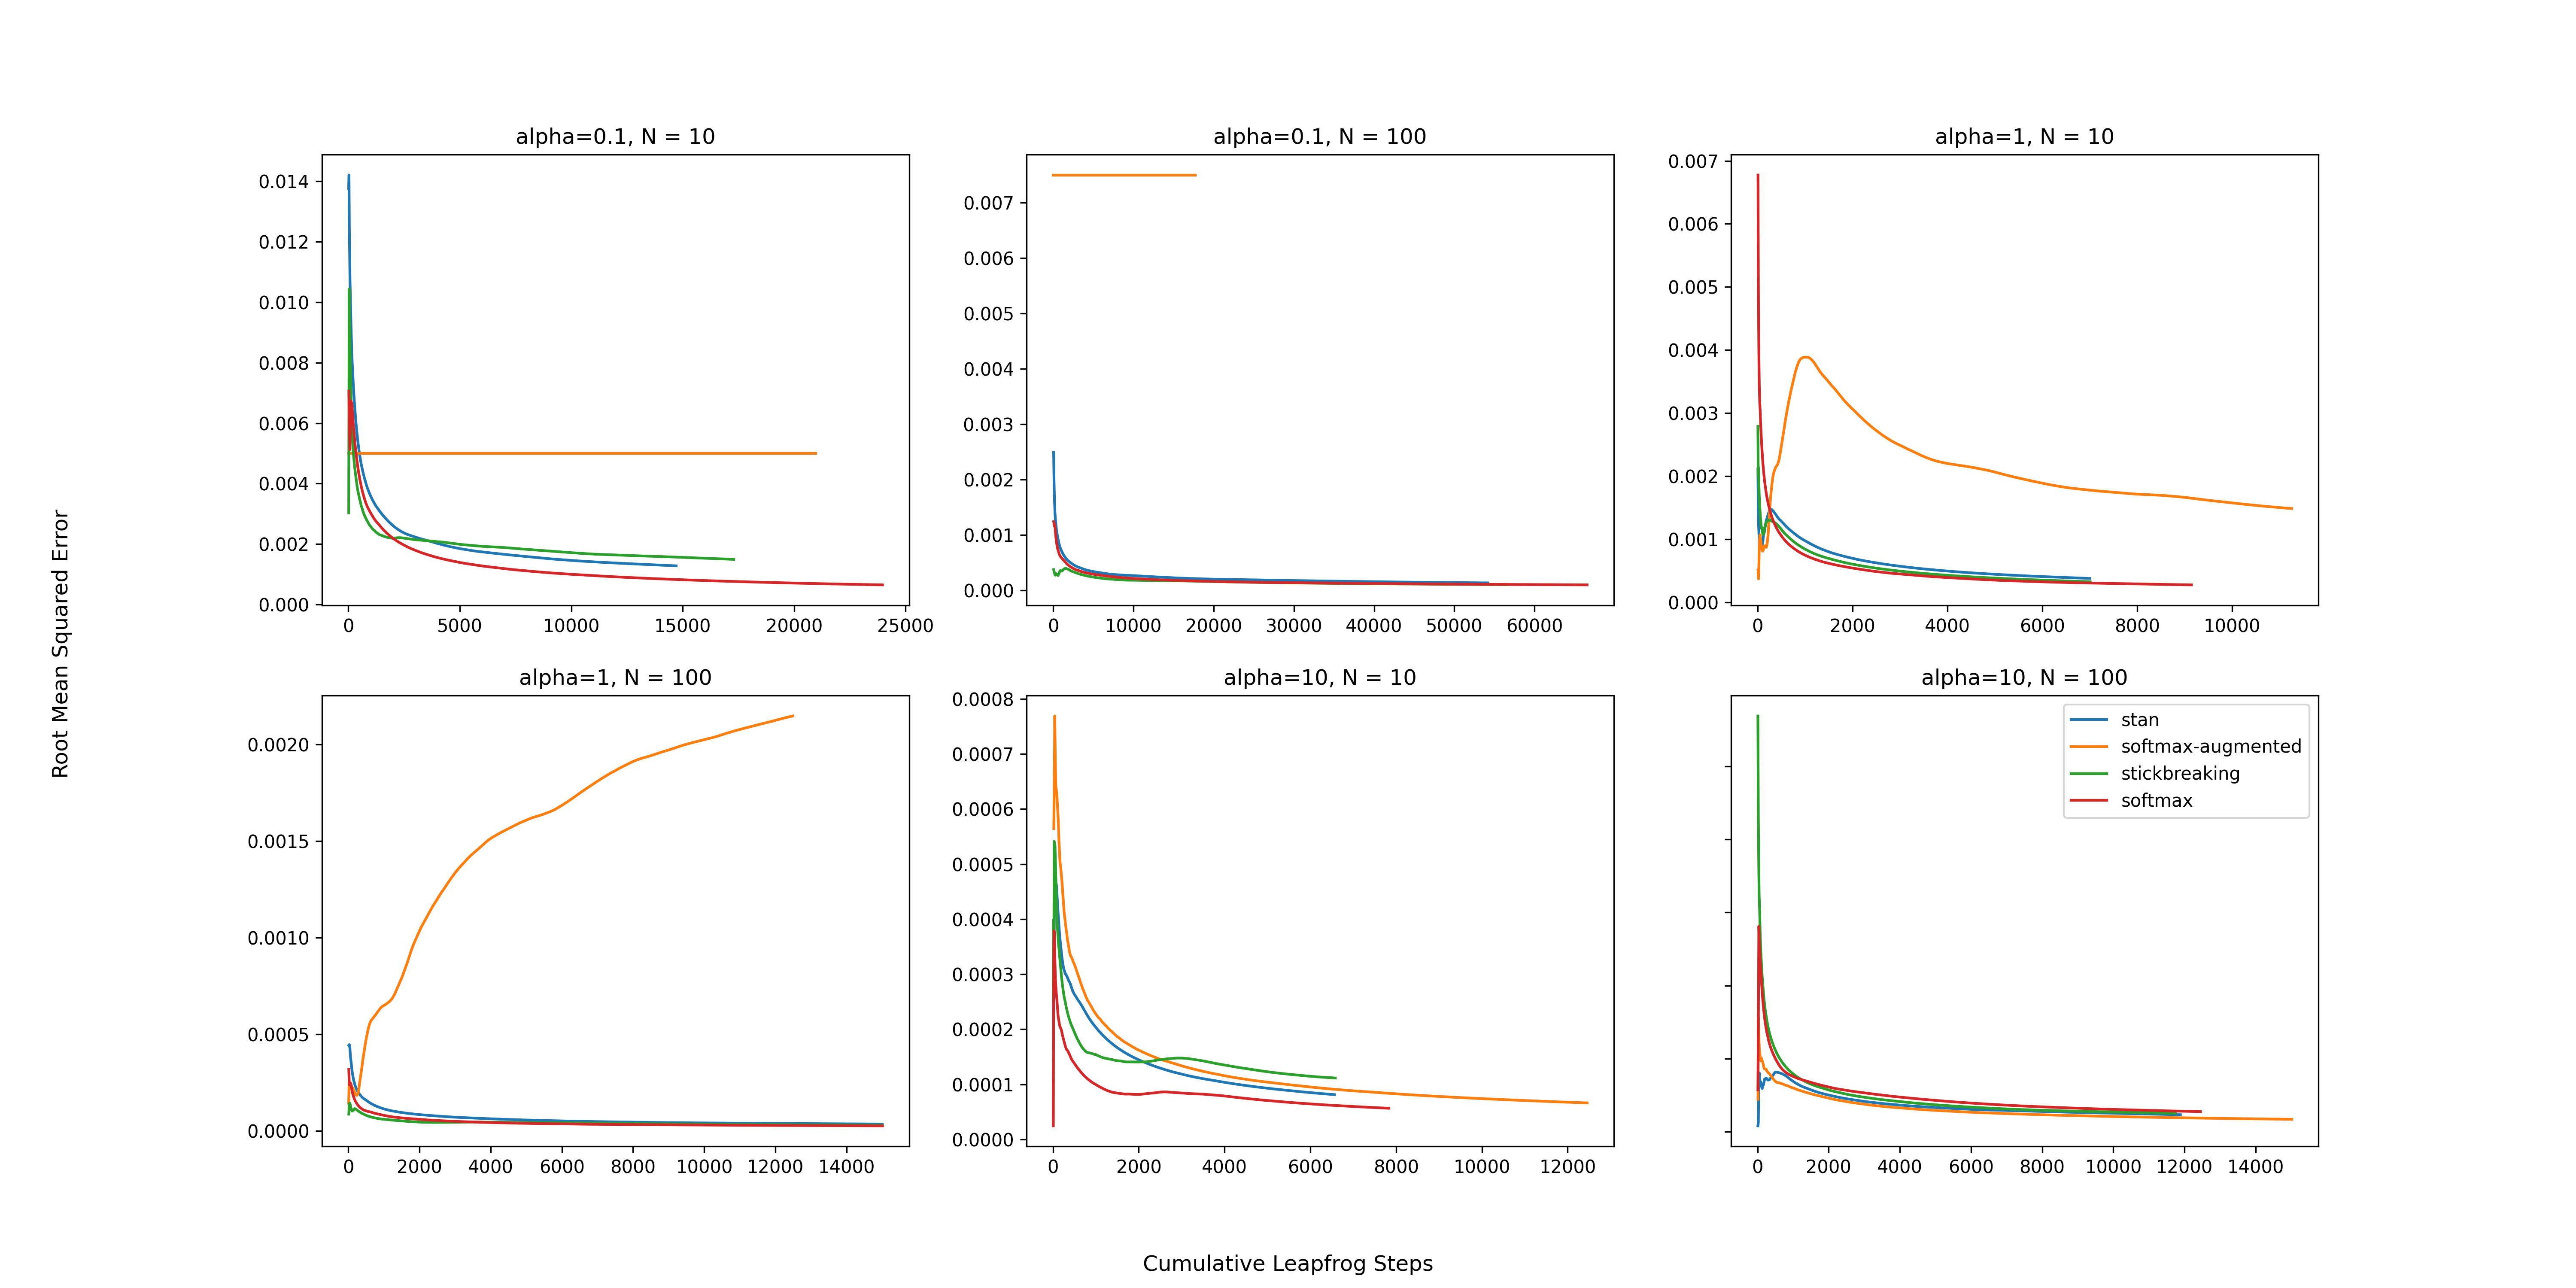
\includegraphics[width=1.2\textwidth]{figures/rmse.png}
    \caption{Root Mean Squared Error vs Cumulative Leapfrog Steps}
    \label{fig:my_label}
\end{figure}

\subsubsection*{Acknowledgements}

We would like to thank \url{matrixcalculus.org} for providing an
easy-to-use symbolic matrix derivative calculator.



\bibliography{all}{}
\bibliographystyle{plain}

\end{document}
